\subsection{Animacje}
Jednym z głównych komponentów na obiekcie jest Animator.
To dzięki niemu postacie odpowiednio poruszają się podczas zmieniania swojej pozycji lub ataku.
Animator jest odpowiedzialny za wszystkie animacje odgrywane przez nasze postaci, zarówno te sterowane przez komputer, jak i graczy.

    \begin{figure}[H]
    \center
    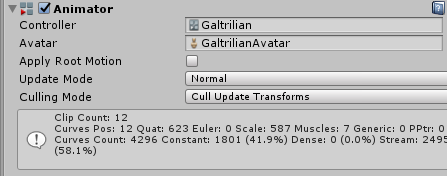
\includegraphics[width=9cm]{animator_4.png}
    \caption{ \textit{Animator}}
    \end{figure}

Składa się on z dwóch ważnych elementów. Jednym z nich jest kontroler, który odpowiada za wszystkie przejścia pomiędzy naszymi animacjami. Odbiera on parametry, które na bieżąco aktualizowane są przez odpowiednie skrypty zaimplementowane dla danego obiektu. Wykrywają one wszystkie sygnały z urządzeń wejścia, odbierają informacje od innych graczy, postaci niekontrolowanych przez użytkowników oraz otoczenia.

Ważną kwestią jest odpowiednie zaprogramowanie kontrolera, gdyż na jego podstawie postać będzie odpowiednio reagować i przemieszczać się. Jeśli jeden z warunków zawiedzie nasz gracz może pozostać w fazie ataku, która nigdy się nie skończy, przez co będzie blokowała wszystkie inne ruchy dla danej postaci.

Podstawą w kontrolerze są stany, a ich głównym parametrem jest Motion. Zawiera informacje o animacji, która ma się wykonać, gdy postać znajduje się w określonym momencie.

\begin{figure}[H]
    \center
    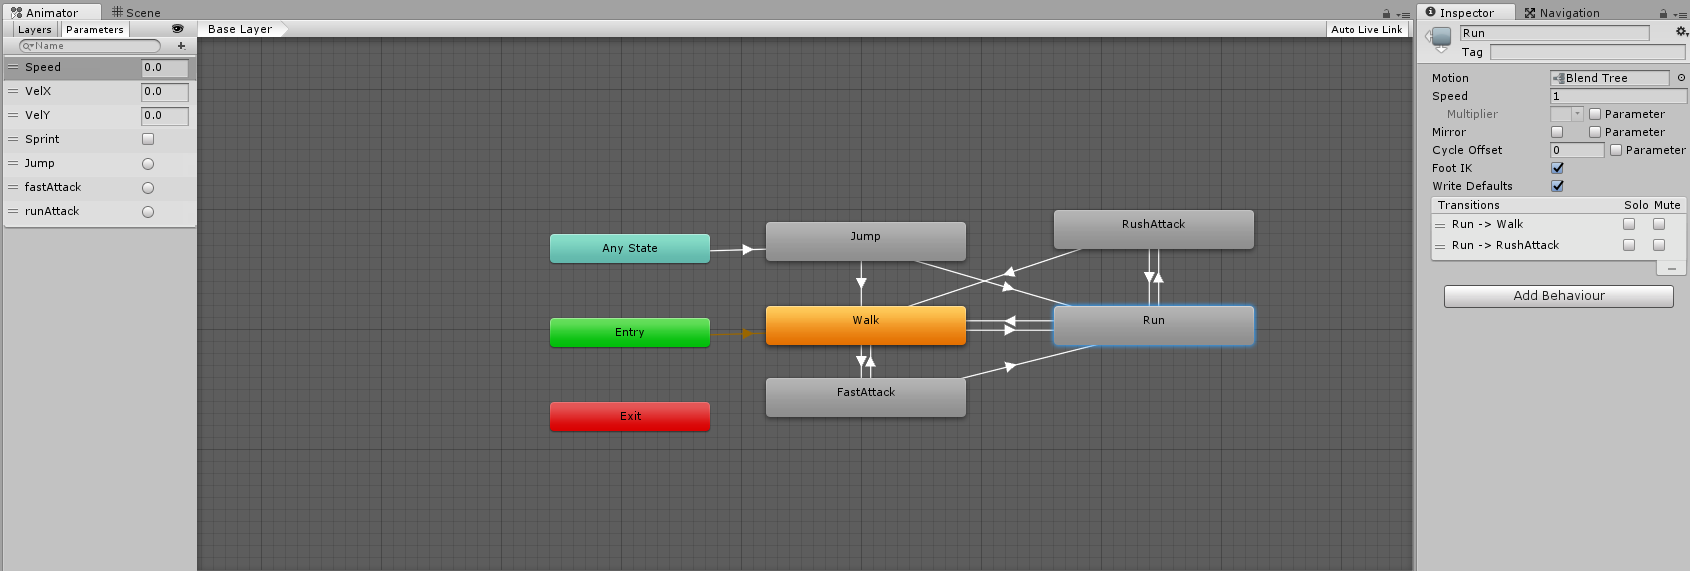
\includegraphics[width=\textwidth]{animator_2.png}
    \caption{ \textit{Stany odpowiadające za animacje wojownika}}
    \end{figure}

Żeby postać mogła przejść z jednego stanu na drugi niezbędne są transakcje. To w nich ustalamy zmianę animacji względem poszczególnych parametrów. 

Zwykłe stany posiadają jednak jedną znaczącą wadę, brak płynnych przejść pomiędzy poszczególnymi animacjami. Postać w jednym momencie po prostu zmienia animacje na kolejną, co bardzo psuje efekt wizualny. Aby uniknąć tego w naszym projekcie użyliśmy bardziej zaawansowanej opcji – Blend Tree.

Blend Tree to bardziej rozbudowane stany, które pozwalają na płynne przejścia pomiędzy animacjami oraz łączenie ich. Dzięki czemu nasza postać może połączyć np. bieg w przód z poruszaniem się na boki. Daje to również odczucie, jakby nasza postać posiadała o wiele więcej animacji.
\begin{figure}[H]
    \center
    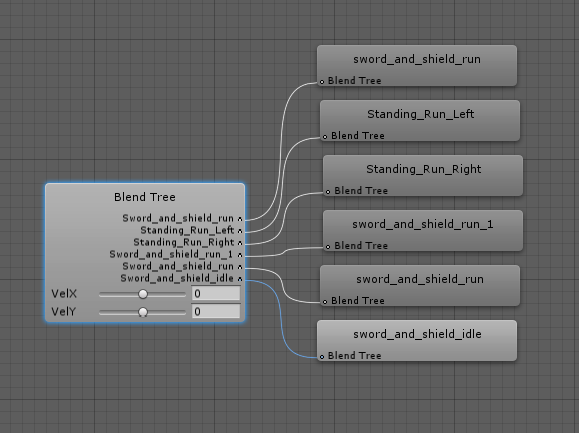
\includegraphics[width=9cm]{blendtree_1.png}
    \caption{ \textit{Stan "Run"  zaimplementowany jako Blend Tree}}
    \end{figure}


W Blend Tree możemy wykorzystać również stopniowe zwiększanie się naszych parametrów. Najlepszy efekt wspomnianej funkcjonalności możemy zaobserwoać w momencie, gdy nasz użytkownik zdecyduje się na sterowanie kontrolerem z gałkami analogowymi, które są czułe na siłę nacisku. Im bardziej gracz będzie przesuwał analog w przód, tym bardziej nasza postać będzie się pochylać i przechodzić płynnie do kolenej animacji.

\begin{figure}[H]
    \center
    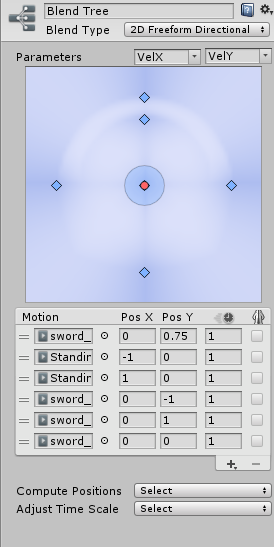
\includegraphics[width=5cm]{blendtree_2.png}
    \caption{ \textit{Przejcia pomiędzy animacjami biegu w Blend Tree, na podstawie parametrów X oraz Y}}
    \end{figure}
